\IfFileExists{.__texlab_dummy}{\bibliography{../texlab_refs}}{}

\section{РЕАЛИЗАЦИЯ И АНАЛИЗ ЭФФЕКТИВНОСТИ МОДЕЛЕЙ}

В практической части работы были реализованы и обучены четыре модели нейронного машинного перевода: LSTM с механизмом внимания, Transformer, Mamba в схеме encoder-decoder и Mamba только с декодером.
LSTM использовалась как базовая рекуррентная модель.
Transformer был выбран как стандартная архитектура машинного перевода с механизмом самовнимания.
Две модели Mamba позволяют сравнить классическую encoder-decoder схему с decoder-only подходом.
Такое сравнение актуально, поскольку Mamba рассматривается как альтернатива self-attention для обработки длинного контекста без квадратичной сложности~\cite{transformer,mtssm}.

Реализация выполнена на языке Python с использованием библиотеки \textbf{PyTorch}.
Для всех моделей использовалась одинаковая схема обучения.
Модели обучались с оптимизатором AdamW, ограничением нормы градиента и функцией потерь cross-entropy с label smoothing.
Планировщик скорости обучения состоял из линейного warmup и последующего косинусного убывания.

Для обучения использовался вычислительный стенд с видеокартой NVIDIA-H100.

\subsection{Датасет и предобработка данных}

Для обучения использовалась русско-английская часть датасета OPUS-100~\cite{opus100}.
OPUS-100 является многоязычным параллельным корпусом, собранным на основе открытых корпусов OPUS.
Русско-английская часть содержит около 1 млн параллельных пар.
Каждый пример датасета представляет собой пару предложений: предложение на русском языке и соответствующий ему перевод на английский язык.

В работе использовались стандартные разбиения датасета на обучающую, валидационную и тестовую части.
Во время обучения длина последовательности ограничивалась 256 токенами.
Такая граница отсекает слишком длинные предложения, которые сильно увеличивают расход памяти, но при этом сохраняет большую часть обычных предложений корпуса.

Для дополнительного контроля качества данных применялись две проверки.
Во-первых, автоматически проверялся язык предложений.
Так выявлялись примеры, где в русской колонке находился не русский текст или наоборот.
Во-вторых, для части пар оценивалась семантическая близость предложений.
Такая проверка нужна потому, что параллельные корпуса могут содержать технический шум: неполные переводы, перепутанные строки, одинаковые предложения на разных языках.

\subsection{Токенизатор}

Для токенизации использовалась subword-модель Unigram~\cite{sentencepiece}.
В отличие от простого разбиения по словам, subword-токенизация позволяет работать с неизвестными словами, редкими формами и морфологически богатыми языками.
Это особенно важно для русского языка, где одно и то же слово может иметь много грамматических форм.

Перед обучением словаря выполнялась нормализация Unicode в форме NFKC.
Далее применялась предварительная токенизация:
\begin{itemize}
    \item пробелы кодировались через metaspace-представление;
    \item знаки препинания выделялись в отдельные токены;
    \item числа разбивались на отдельные цифровые токены.
\end{itemize}

Отдельная обработка чисел и пунктуации важна для перевода.
Числа чаще всего должны переноситься в перевод без изменения, а знаки препинания задают структуру предложения.
Если такие элементы смешивать с соседними словами, модели сложнее научиться переносить их корректно.

Для encoder-decoder моделей использовались специальные токены начала и конца последовательности, padding-токен и токен неизвестного фрагмента.
Для модели только с декодером дополнительно использовался разделитель между исходным предложением и переводом.

\subsection{Используемые метрики}

Качество машинного перевода нельзя надежно оценивать только функцией потерь, поэтому основной метрикой качества в работе является BLEU.
Метрика BLEU сравнивает $n$-граммы машинного перевода с $n$-граммами эталонного перевода~\cite{bleu}:
\begin{equation}
    \operatorname{BLEU} = BP \cdot \exp\left(\sum_{n=1}^{N} w_n \log p_n\right),
\end{equation}
где $p_n$ --- модифицированная точность по $n$-граммам, $w_n$ --- веса, а $BP$ --- штраф за слишком короткий перевод.
В работе BLEU вычислялся с помощью библиотеки SacreBLEU~\cite{sacrebleu}.

Дополнительно учитывалось число параметров модели.
Эта величина важна, потому что две модели с близким качеством перевода могут существенно отличаться по требованиям к памяти и скорости обучения.

\subsection{Архитектуры моделей}

Первой моделью была LSTM encoder-decoder с механизмом внимания.
Encoder является двунаправленным: одна LSTM читает исходное предложение слева направо, вторая --- справа налево.
Decoder генерирует перевод авторегрессионно.
На каждом шаге применяется механизм внимания, который строит контекстный вектор по скрытым состояниям encoder.

Вторая модель построена на архитектуре Transformer.
Encoder использует самовнимание для построения представлений исходного предложения.
Decoder применяет причинное самовнимание к уже сгенерированной части перевода и отдельный слой внимания к выходам encoder.
Эта модель служит сильной нейросетевой базой для сравнения с Mamba.

Третья модель использует Mamba-блоки в схеме encoder-decoder.
В encoder и decoder последовательная обработка выполняется Mamba-блоками, а связь между исходным предложением и переводом задается слоем внимания.
Такой вариант сохраняет привычную для машинного перевода структуру encoder-decoder, но заменяет часть последовательной обработки на блоки Mamba.

Четвертая модель --- Mamba только с декодером.
В этой схеме исходное предложение и перевод рассматриваются как одна авторегрессионная последовательность.
Во время обучения модель получает исходный текст и правильный перевод, но ошибка оптимизации считается только по токенам перевода.
Во время вывода исходное предложение задает префикс, после чего модель продолжает последовательность токенами перевода.

В таблице \ref{tab:configs} приведены основные конфигурации моделей.

\begin{table}[H]
    \centering
    \caption{Основные конфигурации моделей}
    \label{tab:configs}
    \resizebox{0.98\textwidth}{!}{%
    \begin{tabular}{|l|c|c|c|c|}
        \hline
        Модель & Схема & Размер представления & Число слоев & Особенность \\
        \hline
        LSTM & encoder-decoder & 384 & 4 & рекуррентная базовая модель \\
        Transformer & encoder-decoder & 768 & 6+6 & самовнимание и слой внимания к encoder \\
        Mamba & encoder-decoder & 768 & 6+6 & Mamba-блоки и слой внимания к encoder \\
        Mamba decoder-only & только декодер & 512 & 8 & единая авторегрессионная последовательность \\
        \hline
    \end{tabular}}
\end{table}

\subsection{Графики обучения}

Все модели обучались на 100 тыс. итераций с размером батча 100.
Для BLEU использовались 40 проверок на валидационной выборке.

На рисунке \ref{fig:train_loss} показано изменение функции потерь на обучении.
У всех моделей значение функции потерь убывает, что говорит о корректном ходе оптимизации.
Transformer и Mamba в схеме encoder-decoder быстрее достигают меньших значений функции потерь, а LSTM и Mamba только с декодером сходятся более плавно.

\begin{figure}[H]
    \centering
    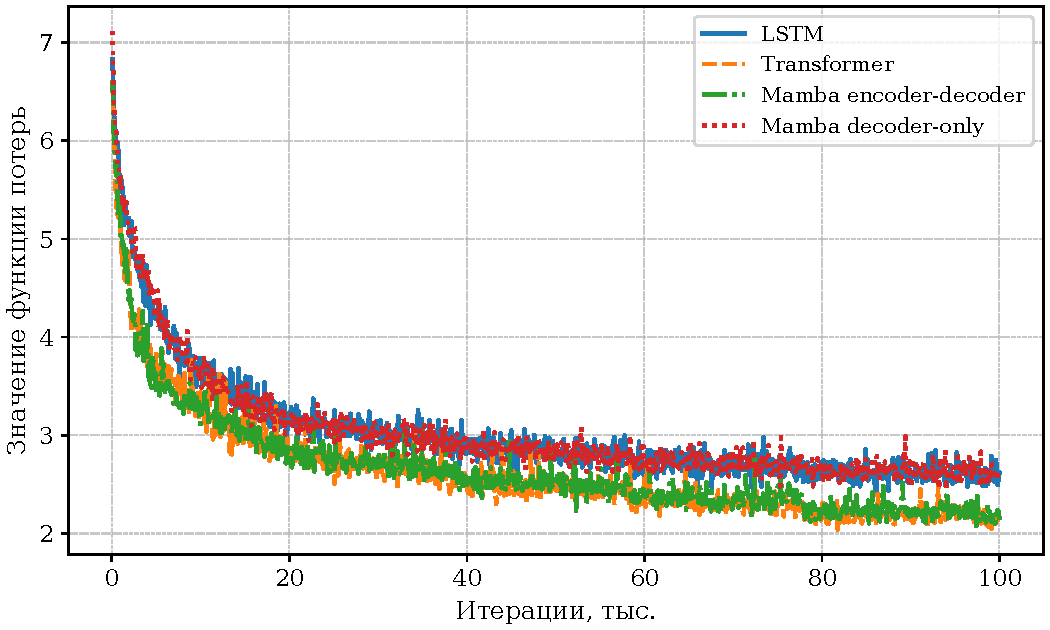
\includegraphics[width=0.88\textwidth]{images/train_loss_successful.pdf}
    \caption{Изменение функции потерь на обучении}
    \label{fig:train_loss}
\end{figure}

На рисунке \ref{fig:validation_bleu} приведено изменение BLEU на валидационной выборке.
По этому графику видно, что Transformer и Mamba encoder-decoder дают близкое качество и заметно превосходят LSTM.
Mamba только с декодером набирает качество медленнее и в данном эксперименте уступает encoder-decoder вариантам.

\begin{figure}[H]
    \centering
    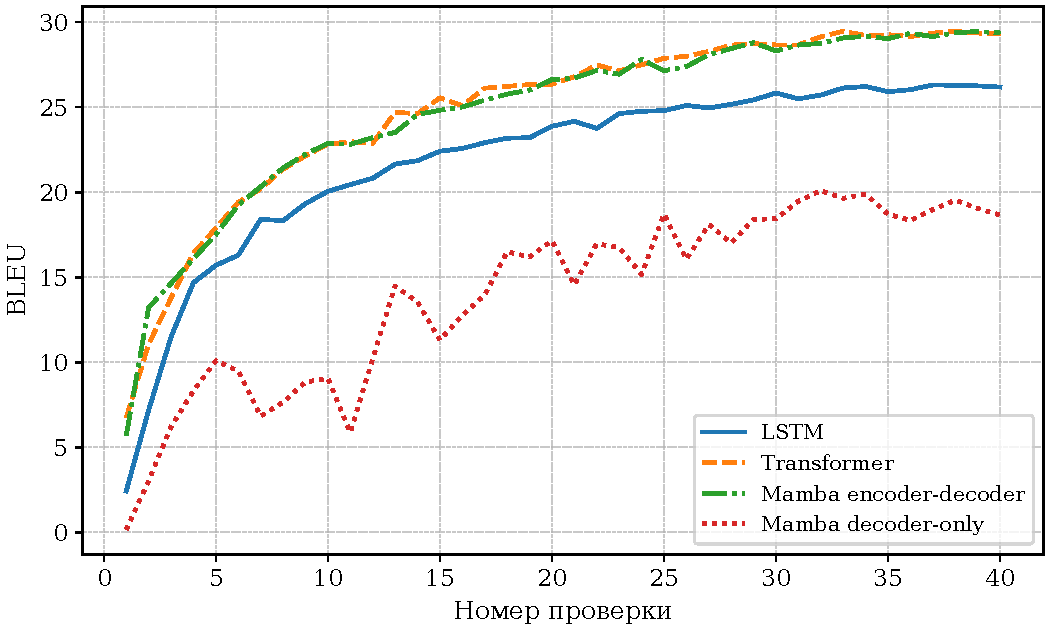
\includegraphics[width=0.88\textwidth]{images/validation_bleu_successful.pdf}
    \caption{Изменение BLEU на валидационной выборке}
    \label{fig:validation_bleu}
\end{figure}

\subsection{Итоговое сравнение}

Итоговые результаты представлены в таблице \ref{tab:results}.
Для BLEU указано лучшее значение на валидационной выборке.
Размер модели указан в миллионах параметров.

\begin{table}[H]
    \centering
    \caption{Итоговое сравнение моделей машинного перевода}
    \label{tab:results}
    \begin{tabular}{|l|c|c|}
        \hline
        Модель & BLEU & Число параметров \\
        \hline
        LSTM & 26.31 & 73.5M \\
        Transformer & 29.47 & 158.8M \\
        Mamba encoder-decoder & 29.45 & 190.3M \\
        Mamba decoder-only & 20.09 & 90.0M \\
        \hline
    \end{tabular}
\end{table}

По результатам видно, что Mamba в схеме encoder-decoder достигает качества, близкого к Transformer, и превосходит LSTM.
При этом вариант Mamba только с декодером показал более низкое значение BLEU.
Это означает, что для рассматриваемого корпуса явное разделение исходного предложения и перевода в encoder-decoder схеме оказалось полезным.
Тем не менее decoder-only вариант остается важным для сравнения, поскольку он показывает, как Mamba работает в единой авторегрессионной постановке задачи.
